\chapter{Andere indexstructuren}\label{ch:andere-indices}
Naast suffixbomen en suffix arrays bestaan er ook nog enkele andere interessante indexstructuren.
We behandelen in dit hoofdstuk de FM-index en de R-index.
Deze maken achterliggend gebruik van suffix arrays, maar zorgen ervoor dat de resulterende index kleiner is.


\section{FM-index}\label{sec:fm-index}
De FM-index~\cite{fm_index} werd als eerste beschreven door Ferragina en Manzini.
Officieel staat de naam voor \textit{Full-text index in Minute space}.
Een FM-index bestaat uit \textbf{3 essentiële componenten}.
De \textbf{Borrows-wheeler transformatie}~\cite{bwt}, \textbf{een (sparse/compressed) suffix array (SA)} en \textbf{bitvectoren} die de rank-operatie ondersteunen.
Het opbouwen van de index voor tekst $T$ kan gebeuren in $O(n)$ tijd, met $n$ de lengte van $T$.
Het zoeken of er een match is, kan in $O(m)$ tijd, met $m$ de lengte van patroon $P$.
Het zoeken inclusief het vinden van waar alle matches in de originele string zitten, kan in $O(m + \text{|occ}(P, T)\text{|} \log n)$.
Hierbij is $\text{occ}(P, T)$ de set van alle indices waar patroon $P$ matcht in de tekst $T$.
In plaats van de originele tekst volledig bij te houden, wordt de BWT van de tekst bijgehouden.
Door de extra informatie die in de BWT verwerkt zit (ten opzichte van de tekst zelf), is het mogelijk om een \textbf{grotere sparseness factor $k$} toe te passen op de SA, zonder dat dit impact heeft op de minimale lengte van zoekbare peptiden.
Zo is het mogelijk om sparseness factor $k = 32$ te gebruiken, waarbij het nog steeds mogelijk is om peptiden die bestaan uit één aminozuur te zoeken, maar dit heeft natuurlijk een negatieve impact op de performantie.
De FM-index laat dus toe om een \textbf{kleinere index} te bekomen, door het gebruik van een hogere sparseness factor $k$ op de SA, zonder verlies van functionaliteit.
Tot slot kan men via een variant van de FM-index, de bidirectionele FM-index, en door gebruik te maken van zogenaamde \textbf{zoekschema's}, ook \textbf{inexacte matching} ondersteunen waarbij maximaal $x$ mismatches toegelaten zijn.

\subsection{Verschillende implementaties}\label{subsec:verschillende-implementaties}
Om een goed beeld te krijgen over het geheugengebruik tijdens het opbouwen, hebben we verschillende FM-index implementaties getest.
Opnieuw focussen we ons vooral op het geheugengebruik aangezien dit de primaire restrictie is tijdens het opbouwen.
Tabel~\ref{tab:fm_index_building} geef een overzicht van de geteste implementaties.
Omdat ons einddoel bestaat uit het indexeren van UniProtKB, kunnen we ons opnieuw enkel focussen op de 64-bit implementaties.
UniProtKB bevat namelijk meer tekens dan door de maximale 32-bit integer voorgesteld kan worden.
Als referentie maken we gebruik van de resultaten uit Tabel~\ref{tab:sa_building}.
Hieruit konden we concluderen dat er 1.86 GB RAM nodig is om een suffix array op te bouwen (met 64-bit integers).
Wanneer we dit vergelijken met de resultaten voor de geteste FM-index implementaties, zien we dat deze \textbf{bijna twee maal zo veel geheugen nodig hebben}.
Zelfs wanneer een sparseness factor geïntroduceerd wordt, zal dit steeds in een hoger geheugengebruik resulteren dan bij een suffix array.
De volledige suffix array is namelijk nodig om efficiënt de BWT af te leiden.
Bovendien moeten we op basis van deze BWT nog een bitvector bijhouden voor elk teken in ons alfabet, behalve voor het unieke eindteken.
Voor UniProtKB zou dit willen zeggen dat er al ongeveer $\frac{88 \cdot 27}{8} \approx 300$ GB RAM nodig hebben enkel hiervoor.
Bovendien moeten deze bitvectoren ook allemaal de rank operatie ondersteunen.
Dit kan efficiënt met ongeveer nog eens 25\% extra geheugen via het rank9 algoritme~\cite{CCB_course, rank9}.
Hierdoor loopt het extra geheugengebruik op tot ongeveer 375 GB\@.
Om die reden hebben we in het kader van deze masterproef deze optie niet verder verkend.

\begin{table}[H]
    \begin{minipage}{\linewidth}
        \centering
        \resizebox{\textwidth}{!}{
            \begin{tabular}{l l S[table-format=-2.2] S[table-format=-2.2] S[table-format=-1.2] S[table-format=-1.2]}
                Implementatie & Programmeertaal & \multicolumn{2}{c}{Tijd (in s)} & \multicolumn{2}{c}{Geheugen (in GB)} \\
                \hline\hline
                &                         & {32-bit} & {64-bit} & {32-bit} & {64-bit} \\
                \cline{3-6}
                \url{https://crates.io/crates/fm-index}     & Rust                    & {-}      & 33.92    & {-}      & 3.22     \\
                \url{https://github.com/simongog/sdsl-lite} & C++                     & {-}      & 27.74    & {-}      & 3.70     \\
                \url{https://github.com/ocfnash/FM-Index}   & Cython met C++ bindings & 57.94    & {-}      & 1.96     & {-}      \\
                \hline
            \end{tabular}
        }
        \caption{Uitvoeringstijd en maximaal geheugengebruik voor het opbouwen van een FM-index voor de Swiss-Prot proteïnedatabank aan de hand van verschillende implementaties.
        Afhankelijk van de gebruikte implementatie (32- of 64-bit) is een andere kolom ingevuld.
        Een - staat voor niet getest. Deze testen werden lokaal uitgevoerd op een M1 Pro MacBook Pro.
        De specificaties hiervan zijn terug te vinden in tabel~\ref{tab:macbook_hardware}.}
        \label{tab:fm_index_building}
    \end{minipage}
\end{table}


\section{R-index}\label{sec:r-index}
R-indices~\cite{r_index2, r_index1} zijn een verdere evolutie van de FM-index waarbij \textbf{run-length encoding (RLE)} toegepast wordt op de \textbf{BWT van de tekst}.
De index heeft grootte $O(r)$ met $r$ het aantal BWT runs van de tekst van lengte $n$.
Vanwege het gebruik van RLE op de BWT, zal de \textbf{resulterende index kleiner} zijn naarmate er \textbf{meer herhaling} voorkomt in de geïndexeerde tekst.
Om na te gaan wat het effect hiervan is op onze proteïnedatabanken, hebben we de R-index getest op de eerste 0.5\%, 1\%,\ldots\space van de volledige UniProtKB databank.
Figuur~\ref{fig:sa_vs_r_index} visualiseert het geheugengebruik en de resulterende indexgrootte in vergelijking met suffix arrays.
Merk op dat het geheugengebruik tijdens het opbouwen en de grootte van de resulterende R-index meer dan verdubbelt bij het overgaan van 2\% (1\thinspace651\thinspace521\thinspace046 tekens) naar 4\% (3\thinspace319\thinspace904\thinspace170 tekens) van UniProtKB\@.
De oorzaak hiervan is het overschakelen van 32-bit naar 64-bit integers binnen de R-index.
Bij de indices tot en met 2\% van UniProtKB maakt de R-index implementatie gebruik van 32-bit integers omdat er minder tekens in de geïndexeerde tekst staan dan de maximale 32-bit integer waarde.
Bij grotere databanken wordt deze 32-bit integer limiet overschreden, waardoor de R-index implementatie moet overschakelen naar het gebruik van 64-bit integers.
\\ \\
Enerzijds valt duidelijk te zien dat het opbouwen van een \textbf{suffix array minder geheugen vraagt}.
Anderzijds is de \textbf{resulterende R-index kleiner}, en wordt deze bovendien procentueel kleiner voor grotere databanken.
Dit is de winst die verkregen wordt door het gebruik van de run-length encoding op de BWT\@ van de tekst.
Natuurlijk zouden we bij de suffix array ook vrij simpel de resulterende index kunnen verkleinen door de SA sparse te maken.
Hierbij zal op een gegeven punt de winst in indexgrootte erg klein zijn omdat de volledige tekst altijd opgeslagen moet worden.
Bij het gebruik van sparseness factor $k = 3$ voor de grootste geteste index zou de totale index voor de suffix array teruggedrongen worden tot 15.31 GB\@.
Van deze 15.31 GB is 4.17 GB de tekst zelf.
Merk op dat de grootte van de resulterende index voor suffix arrays dan nog steeds lineair zal stijgen als de databank groeit, maar met een kleinere constante.
Aangezien de \textbf{resulterende indexgrootte voor R-indices sublineair stijgt}, zullen we de sparseness factor $k$ van suffix arrays groter en groter moeten maken om een even kleine resulterende index te hebben.
Dit maakt een R-index op dit vlak een interessante indexstructuur voor grote proteïnedatabanken.
\\ \\
Opnieuw is het geheugengebruik tijdens het opbouwen hier een sterk beperkende factor.
Dit geheugengebruik is meer dan twee keer zo groot als bij het bouwen van een suffix array, waardoor we deze optie niet verder zullen verkennen.
Bovendien kunnen we door het gebruik van een hogere sparseness factor de resulterende suffix array toch snel twee tot drie maal kleiner maken, zonder al te veel performantieverlies.

\begin{figure}[H]
    \centering
    \subfloat[Maximaal geheugengebruik tijdens het opbouwen van een suffix array en R-index.]{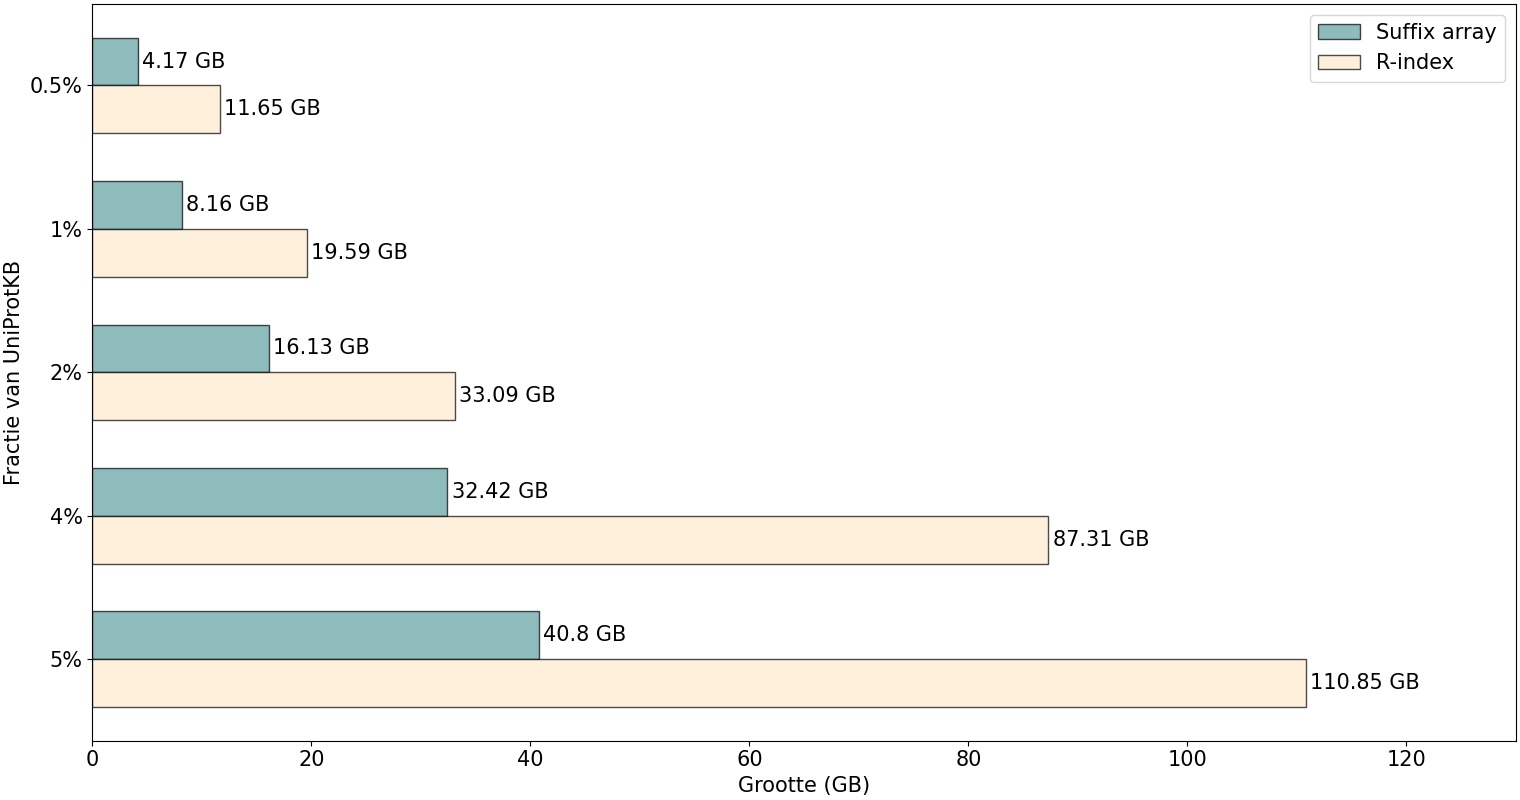
\includegraphics[width=0.8\linewidth]{sa_vs_r_index_build_memory}}\\[4ex] % [4ex] om wat extra vertical spacing in te voegen

    \subfloat[Resulterende indexgrootte voor een suffix array (sparseness factor $k = 1$) en R-index.]{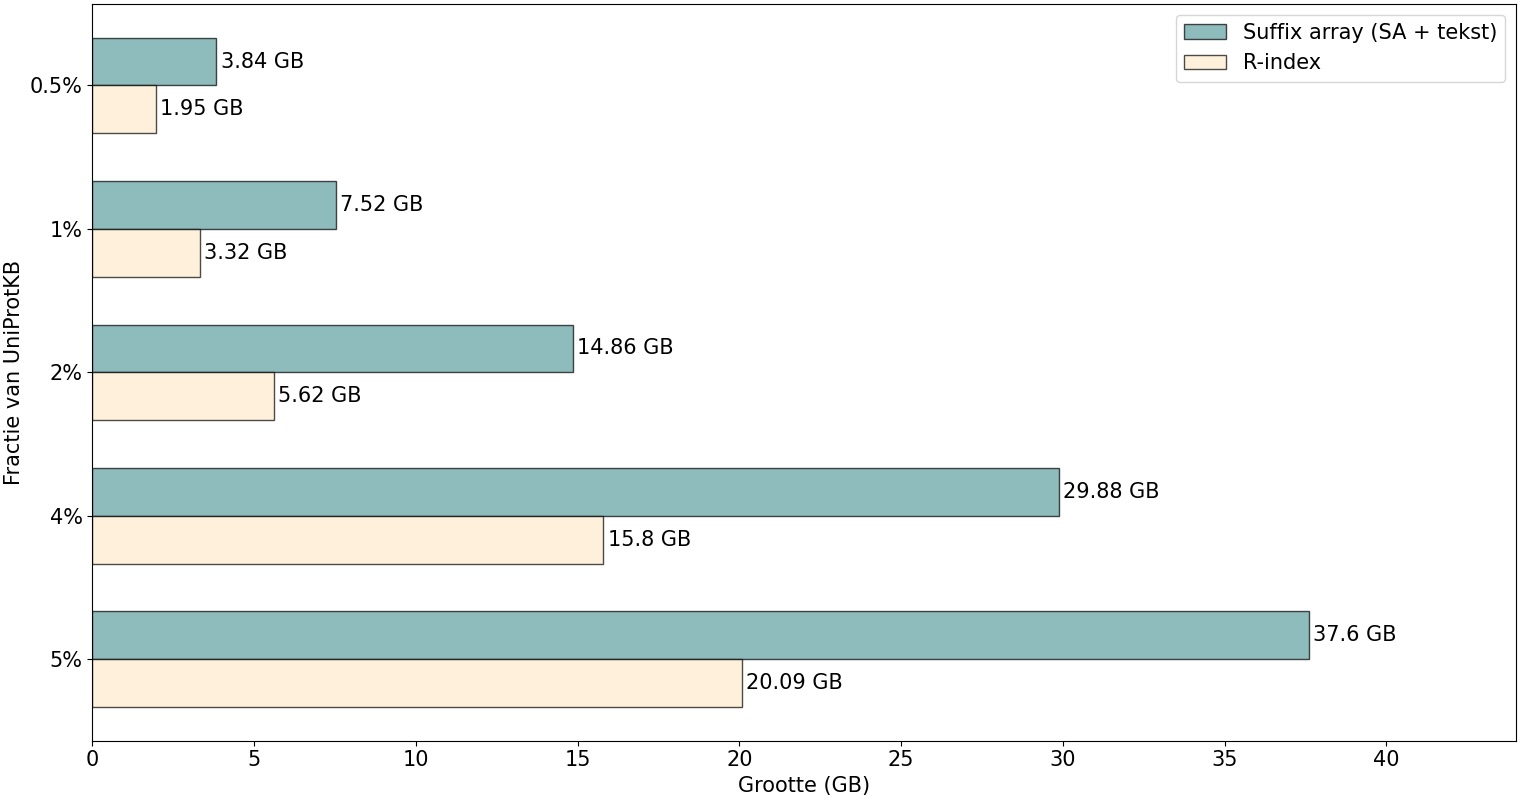
\includegraphics[width=0.8\linewidth]{sa_vs_r_index_index_memory}}
    \caption{Vergelijking van de suffix array en R-index op vlak van geheugengebruik en de resulterende indexgrootte voor verschillende deelverzamelingen van UniProtKB. Bij elke test gaat het om de eerst $x$ procent van de database. Bij de suffix array wordt sparseness factor $k = 1$ gebruikt. Het gebruik van een andere sparseness factor heeft enkel invloed op de grootte van de resulterende index.}\label{fig:sa_vs_r_index}
\end{figure}


